% Copyright (C) 2014 Miquel Sabaté Solà <mikisabate@gmail.com>
% This file is licensed under the MIT license.
% See the LICENSE file.

\section{Planning}

\subsection{Project planning and feasability}

The first period of the project is dedicated to studying the feasability of the
project and to do the initial planning of the project. This is done through a
course called GEP, that is currently running. This course includes the
following stages:

\mylist
  \item Scope of the project.
  \item Project planning.
  \item Budget and sustainability.
  \item Preliminary presentation.
  \item Bibliography.
  \item List of conditions.
  \item Oral presentation and delivery of the final document.
\mylistend

\subsection{Project analysis and design}

The main goal of this stage is to draw a clear picture of the project and
analyze all the goals of the project. After doing this, I will move my efforts
towards the design of the application.

Therefore, this stage is made out of two sub stages. The first one, the
analysis of the project. In this sub stage I will be defining all the goals,lose
requirements, features and use cases of my application.

The other sub stage consists in design the application. This will be done by
creating diagrams, drawing flow charts, etc.

\subsection{Project iterations}

\begin{enumerate}
 \item {\bf Development of the core software infrastructure}

 In this iteration I am going to focus on the core infrastructure that has to
hold the whole application. This will be executed only in the software front.
I will consider that this stage has ended when there is production-ready base
software that can hold the infrastructure and that is well documented and
thoroughly tested.

 \item {\bf Providing services}

 The next iteration consists of building services on top of the base
infrastructure that has been created in the previous stage. Similarly to the
previous stage, all the services build at this point will be documented and
tested consciously.

  \item {\bf Designing the cluster}

  At this point, we have the software ready to be put in production. Now we
need to design and implement a cluster that can hold the software. In this
stage I will be using lots of concepts learnt at the university, specially from
the CPD course.

  \item {\bf Concluding the development}

  In the last iteration I will be concluding the development of this project.
It consists of doing final tests on both the software and the hardware. This
last iteration will be used to make sure that everything runs smoothly.
\end{enumerate}


\subsection{Final stage}

The final stage consists on closing the project. Since all the code and the
cluster design has already been set up to this point, I am just going to focus
on the following topics:

\mylist
  \item Documentation.
  \item Final report.
  \item Final presentation.
\mylistend

\section*{Gantt chart}

\begin{center}
  \hspace*{-2cm}
  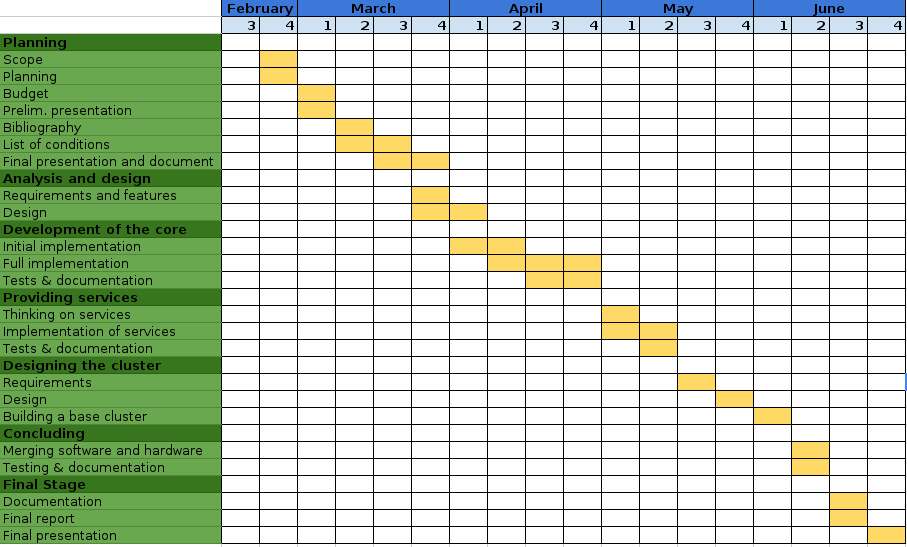
\includegraphics[scale=0.75]{images/gantt.png}
\end{center}

I don't like to compute the work to be done in hours. I prefer to do it in
weeks. In the Gantt chart we can see the scheduling that I've made for the
project divided by weeks. Some tasks are overlapping in some weeks. This is
quite normal.

The total amount of hours is not fixed, it depends on the work that is needed
to be done for each task. The important thing here is that we make the
deadlines with no problems.

\subsection{Action plan}

At this point, it is clear how the stages are scheduled. Now, what happens if
any stage has a different duration than expected ? In my case, I will just
start the next stage. That is, if I will start each stage as soon as possible.

In the end of each stage I will do an evaluation of the work done so far. This
will allow me to rearrange the schedule so I don't lose the track of the
development of the project.

Moreover, at the end of each iteration I will meet with my director to analyze
how is the project going. This will force me to work hard to meet the deadlines
and it will also give me the oportunity to have some feedback from the director.
